\chapter{\textbf{\uppercase{Three-band Tight-binding Model for TMDs}}}
In this chapter, based on the tight-binding framework introduced in Chapter~2, we adopt the model developed by Liu \textit{et al.}~\cite{PhysRevB.88.085433}, which constructs a minimal three-band model using three transistion metal orbitals as the basis. This model is commonly referred to as the three-band tight-binding model. Next, we extend this model to include the effects of an external magnetic field by using the Peierls substitution. Finally, we derive the Hamiltonian in the presence of the magnetic field.
\section{Three-band tight-binding model without magnetic field}\label{Section 3.1}

We take MoS$_2$ as a representative example and, based on previous \textit{ab initio} calculations, observe that at high-symmetry points in the Brillouin zone, specifically $\Gamma$, $K$, and $M$, the regions near the highest valence band and lowest conduction band are primarily contributed by the molybdenum $d_{z^2}$, $d_{xy}$, and $d_{x^2 - y^2}$ orbitals. In contrast, the $d_{xz}$, $d_{yz}$ orbitals of molybdenum and the $p_x$, $p_y$, and $p_z$ orbitals of sulfur contribute mainly to higher-energy subbands. This indicates that the low-energy bands near the band gap are predominantly governed by the $d_{z^2}$, $d_{xy}$, and $d_{x^2 - y^2}$ orbitals.  

Since only the orbitals of the M atom are included, we ignore the sum over atomic positions $\mathbf{r}_i$ within the unit cell in Eq.~(2.3), and denote the wave functions of the three orbitals of the M atom as
\begin{gather}
	\ket{\phi_{1}} = \ket{d_{z^{2}}} , \quad \ket{\phi_{2}} = \ket{d_{xy}} , \quad \ket{\phi_{3}} = \ket{d_{x^{2} - y^{2}}}.
\end{gather}
The Bloch wavefunction in this model has the form
\begin{gather}
	\psi_{\lambda,\mathbf{k}}(\mathbf{r}) = \sum_{j=1}^{3} C_{j}^{\lambda}(\mathbf{k}) \sum_{\mathbf{R}} e^{i \mathbf{k \cdot R}} \phi_{j}(\mathbf{r} - \mathbf{R}).
\end{gather}
The coefficents $C_{j}^{\lambda}(\mathbf{k})$ are the solutions of the eigenvalue equation
\begin{gather}
	\sum_{jj'}^{3} \left[H_{jj'}^{\text{TB}}(\mathbf{k}) - \varepsilon_{\lambda}(\mathbf{k}) S_{jj'}(\mathbf{k})\right] C_{j}^{\lambda}(\mathbf{k}) = 0,
\end{gather}
where
\begin{equation}
	\begin{aligned}
		H_{jj'}^{\text{TB}}(\mathbf{k}) = \sum_{\mathbf{R}} e^{i \mathbf{k \cdot R}} \bra{\phi_{j}(\mathbf{r})} \left[-\f{\hbar^{2} \nabla^{2}}{2m} + U_{0}(\mathbf{r})\right] \ket{\phi_{j'}(\mathbf{r - R})},
	\end{aligned}
\end{equation}
and
\begin{equation}
	\begin{aligned}
		S_{jj'}(\mathbf{k}) = \sum_{\mathbf{R}} \bra{\phi_{j}(\mathbf{r})} \ket{\phi_{j'}(\mathbf{r - R})} \approx \delta_{jj'}.
	\end{aligned}
\end{equation}

Take into account up to \ac{TNN} hopping, the matrix elements of the \ac{TB} Hamiltonian Eq.~(3.4) are
\begin{equation}
	\begin{aligned}
		H_{jj'}^{\text{TNN}}(\mathbf{k})
		& = \mathcal{E}_{jj'}(\mathbf{0}) + e^{i\mathbf{k}\cdot \mathbf{R}_{1}}\mathcal{E}_{jj'}(\mathbf{R}_{1}) + e^{i\mathbf{k}\cdot \mathbf{R}_{2}}\mathcal{E}_{jj'}(\mathbf{R}_{2}) + e^{i\mathbf{k}\cdot \mathbf{R}_{3}}\mathcal{E}_{jj'}(\mathbf{R}_{3})                 \\
		& + e^{i\mathbf{k}\cdot \mathbf{R}_{4}}\mathcal{E}_{jj'}(\mathbf{R}_{4}) + e^{i\mathbf{k}\cdot \mathbf{R}_{5}}\mathcal{E}_{jj'}(\mathbf{R}_{5}) + e^{i\mathbf{k}\cdot \mathbf{R}_{6}}\mathcal{E}_{jj'}(\mathbf{R}_{6})                                                 \\
		& + e^{i\mathbf{k}\cdot \tilde{\mathbf{R}}_{1}}\mathcal{E}_{jj'}(\tilde{\mathbf{R}}_{1}) + e^{i\mathbf{k}\cdot \tilde{\mathbf{R}}_{2}}\mathcal{E}_{jj'}(\tilde{\mathbf{R}}_{2}) + e^{i\mathbf{k}\cdot \tilde{\mathbf{R}}_{3}}\mathcal{E}_{jj'}(\tilde{\mathbf{R}}_{3}) \\
		& + e^{i\mathbf{k}\cdot \tilde{\mathbf{R}}_{}4}\mathcal{E}_{jj'}(\tilde{\mathbf{R}}_{4}) + e^{i\mathbf{k}\cdot \tilde{\mathbf{R}}_{5}}\mathcal{E}_{jj'}(\tilde{\mathbf{R}}_{5}) + e^{i\mathbf{k}\cdot \tilde{\mathbf{R}}_{6}}\mathcal{E}_{jj'}(\tilde{\mathbf{R}}_{6}) \\
		& + e^{i\mathbf{k}\cdot 2\mathbf{R}_{1}}\mathcal{E}_{jj'}(2\mathbf{R}_{1}) + e^{i\mathbf{k}\cdot 2\mathbf{R}_{2}}\mathcal{E}_{jj'}(2\mathbf{R}_{2}) + e^{i\mathbf{k}\cdot 2\mathbf{R}_{3}}\mathcal{E}_{jj'}(2\mathbf{R}_{3})                                           \\
		& + e^{i\mathbf{k}\cdot 2\mathbf{R}_{4}}\mathcal{E}_{jj'}(2\mathbf{R}_{4}) + e^{i\mathbf{k}\cdot 2\mathbf{R}_{5}}\mathcal{E}_{jj'}(2\mathbf{R}_{5}) + e^{i\mathbf{k}\cdot 2\mathbf{R}_{6}}\mathcal{E}_{jj'}(2\mathbf{R}_{6}) ,                                          \\
	\end{aligned}
\end{equation}
where
\begin{gather}
	\mathcal{E}_{jj'}(\mathbf{R}) = \bra{\phi_{j}(\mathbf{r})} \left[-\frac{\hbar \nabla^{2}}{2m} + U_{0} (\mathbf{r})\right] \ket{\phi_{j'}(\mathbf{r-R})},
\end{gather}
and $\mathbf{R}_{i}, \tilde{\mathbf{R}}_{i}$ and $2\mathbf{R}_{i}$ are one of the \ac{NN}, \ac{NNN} and third-nearest-neighbor (TNN) vectors, respectively, where $i = 1,...,6$, see in Fig.~3.1. In Table~3.1, we summarize the coordinates of hopping vectors considered in the model.
\begin{table}[h]
	\label{Table 2.1}
	\begin{equation*}
		\renewcommand{\arraystretch}{1.5}
		\begin{NiceArray}{c c c}
			\hline
			\hline
			\text{Vector}          & \text{Hopping relative coordinates} & \text{Cartesian's coordinates}                    \\
			\hline
			\mathbf{R}_{1}         & (m,n) \to (m+2,n)                   & a (1,0,0)                                         \\
			\mathbf{R}_{2}         & (m,n) \to (m+1,n-1)                 & a \left(\frac{1}{2},-\frac{\sqrt{3}}{2},0\right)  \\
			\mathbf{R}_{3}         & (m,n) \to (m-1,n-1)                 & a \left(-\frac{1}{2},-\frac{\sqrt{3}}{2},0\right) \\
			\mathbf{R}_{4}         & (m,n) \to (m-2,n)                   & a (-1,0,0)                                        \\
			\mathbf{R}_{5}         & (m,n) \to (m-1,n+1)                 & a \left(-\frac{1}{2},\frac{\sqrt{3}}{2},0\right)  \\
			\mathbf{R}_{6}         & (m,n) \to (m+1,n+1)                 & a \left(-\frac{1}{2},\frac{\sqrt{3}}{2},0\right)  \\
			\tilde{\mathbf{R}}_{1} & (m,n) \to (m+3,n-1)                 & l \left(\frac{\sqrt{3}}{2},-\frac{1}{2},0\right)  \\
			\tilde{\mathbf{R}}_{2} & (m,n) \to (m,n-2)                   & l \left(0,-1,0\right)                             \\
			\tilde{\mathbf{R}}_{3} & (m,n) \to (m-3,n-1)                 & l \left(-\frac{\sqrt{3}}{2},-\frac{1}{2},0\right) \\
			\tilde{\mathbf{R}}_{4} & (m,n) \to (m-3,n+1)                 & l \left(-\frac{\sqrt{3}}{2},\frac{1}{2},0\right)  \\
			\tilde{\mathbf{R}}_{5} & (m,n) \to (m,n+2)                   & l \left(0,-1,0\right)                             \\
			\tilde{\mathbf{R}}_{6} & (m,n) \to (m+3,n+1)                 & l \left(\frac{\sqrt{3}}{2},\frac{1}{2},0\right)   \\
			2\mathbf{R}_{1}        & (m,n) \to (m+4,n)                   & a (2,0,0)                                         \\
			2\mathbf{R}_{2}        & (m,n) \to (m+2,n-2)                 & a (1,-\sqrt{3},0)                                 \\
			2\mathbf{R}_{3}        & (m,n) \to (m-2,n-2)                 & a (-1,-\sqrt{3},0)                                \\
			2\mathbf{R}_{4}        & (m,n) \to (m-4,n)                   & a (-2,0,0)                                        \\
			2\mathbf{R}_{5}        & (m,n) \to (m-2,n+2)                 & a (-1,\sqrt{3},0)                                 \\
			2\mathbf{R}_{6}        & (m,n) \to (m+2,n+2)                 & a (1,\sqrt{3},0)                                  \\
			\hline
			\hline
		\end{NiceArray}
	\end{equation*}
	\caption[Coordinates relative of hopping terms.]{Hopping vectors used in the model and their hopping respective relative coordinates to the original site $(m,n)$, where $a = 3.190$ \AA \;is lattice constant and $l = a\sqrt{3}$.}
\end{table}
%\begin{equation}
%\begin{aligned}
%	\mathbf{R}_{1} & = (a,0), \quad \mathbf{R}_{2} = \left(\f{a}{2}, - \f{a\sqrt{3}}{2}\right), \quad \mathbf{R}_{3} = \left(-\f{a}{2},-\f{a\sqrt{3}}{2}\right), \\
%	\mathbf{R}_{4} & = (-a,0), \quad \mathbf{R}_{5} = \left(-\f{a}{2}, \f{a\sqrt{3}}{2}\right), \quad \mathbf{R}_{6} = \left(\f{a}{2},\f{a\sqrt{3}}{2}\right).
%\end{aligned}
%\end{equation}
%Here, $\mathbf{R}_{1-6}$ are the positions of the nearest neighbors M atoms, see Fig. 2.1
\begin{figure}[H]
	\centering
	\includegraphics[width=\linewidth]{pic/schematicLatticeTNN.pdf}
	\caption[The hexagonal structure with neighbor hoppings.]{\label{fig:Lattice vectors}The hexagonal structure of the monolayer \ac{TMD} with the metal atoms at the green larger circles and the chalcogen atoms at the smaller yellow circles. The solid red, dash blue and dot purple arrows prepresent the \ac{NN} ($\mathbf{R}_{i}$), \ac{NNN} ($\tilde{\mathbf{R}}_{i}$) and \ac{TNN} (2$\mathbf{R}_{i}$), respectively, and $\mathbf{R}$ are lattice vectors, where $i = 1,...,6$.}
\end{figure}
%%%%% Table
\begin{table}[h]
	\begin{equation*}
		\renewcommand{\arraystretch}{1.5}
		\begin{NiceArray}{c c c c c c c}
			\hline
			\hline
			g_{n}                  & x'                                   & y'                                  & z' & z'^{2} & x'y'                                               & \frac{1}{2}(x'^{2} - y'^{2})                        \\
			\hline
			E                      & x                                    & y                                   & z  & z^{2}  & xy                                                 & \frac{1}{2}(x^{2} - y^{2})                          \\
			C_{3}(\frac{-2\pi}{3}) & -\frac{1}{2}x + \frac{\sqrt{3}}{2} y & -\frac{\sqrt{3}}{2}x - \frac{1}{2}y & z  & z^{2}  & -\frac{1}{2}xy + \frac{\sqrt{3}}{4}(x^{2} + y^{2}) & -\frac{\sqrt{3}}{2} xy - \frac{1}{4}(x^{2} - y^{2}) \\
			C_{3}(\frac{-4\pi}{3}) & -\frac{1}{2}x - \frac{\sqrt{3}}{2} y & \frac{\sqrt{3}}{2}x + \frac{1}{2}y  & z  & z^{2}  & -\frac{1}{2}xy - \frac{\sqrt{3}}{4}(x^{2} + y^{2}) & \frac{\sqrt{3}}{2} xy - \frac{1}{4}(x^{2} - y^{2})  \\
			C_{2}(-\pi)            & -x                                   & -y                                  & z  & z^{2}  & xy                                                 & \tfrac{1}{2}(x^{2} - y^{2})                         \\
			\sigma_{\nu}           & -x                                   & y                                   & z  & z^{2}  & -xy                                                & \frac{1}{2}(x^{2} - y^{2})                          \\
			\sigma'_{\nu}          & \frac{1}{2}x - \frac{\sqrt{3}}{2}    & -\frac{\sqrt{3}}{2}x - \frac{1}{2}y & z  & z^{2}  & \frac{1}{2}xy - \frac{\sqrt{3}}{4}(x^{2} + y^{2})  & -\frac{\sqrt{3}}{2} xy - \frac{1}{4}(x^{2} - y^{2}) \\
			\sigma''_{\nu}         & \frac{1}{2}x + \frac{\sqrt{3}}{2}    & \frac{\sqrt{3}}{2}x - \frac{1}{2}y  & z  & z^{2}  & \frac{1}{2}xy + \frac{\sqrt{3}}{4}(x^{2} + y^{2})  & \frac{\sqrt{3}}{2} xy - \frac{1}{4}(x^{2} - y^{2})  \\
			\hline
			\hline
		\end{NiceArray}
	\end{equation*}
	\caption[Symmetry operators of the $D_{3h}$ point group.]{Some symmetry operators of the $D_{3h}$ point group on basis functions taking $(x,y,z)$ into $(x',y',z')$. $C_{3}(\frac{-2\pi}{3})$ and $C_{3}(\frac{-4\pi}{3})$ are the rotaions by $\frac{-2\pi}{3}$ and $\frac{-4\pi}{3}$ around the $z$ axis, respectively. $\sigma_{\nu}$ is the reflection angular bisector of $R_{1}$ and $R_{6}$ in Fig. 2.1, and $\sigma'_{\nu},\sigma''_{\nu}$ are obtained through rotating $\sigma_{\nu}$ around the $z$ axis by $2\pi/3$ and $4\pi/3$, respectively.}
\end{table}
%%%%%%%%

One parameterizes the matrices $\mathcal{E}(\mathbf{0}), \mathcal{E}(\mathbf{R}_{1}),\mathcal{E}(\mathbf{\tilde{\mathbf{R}}}_{1}) , \mathcal{E}(\mathbf{\tilde{\mathbf{R}}}_{4})$ and $ \mathcal{E}(2\mathbf{R}_{1})$ by
\begin{equation}
	\renewcommand{\arraystretch}{0.7}
	\begin{aligned}
		\mathcal{E}(\mathbf{0})
		& =
		\begin{pNiceMatrix}
			\epsilon_{1} & 0            & 0            \\
			0            & \epsilon_{2} & 0            \\
			0            & 0            & \epsilon_{2}
		\end{pNiceMatrix},
		\mathcal{E}(\mathbf{R}_{1})
		=
		\begin{pNiceMatrix}
			t_{0}  & t_{1}   & t_{2}  \\
			-t_{1} & t_{11}  & t_{12} \\
			t_{2}  & -t_{12} & t_{22}
		\end{pNiceMatrix},
		\mathcal{E}(2\mathbf{R}_{1})
		=
		\begin{pNiceMatrix}
			u_{0}  & u_{1}   & u_{2}  \\
			-u_{1} & u_{11}  & u_{12} \\
			u_{2}  & -u_{12} & u_{22}
		\end{pNiceMatrix}, \\
		\mathcal{E}(\tilde{\mathbf{R}}_{1})
		& =
		\begin{pNiceMatrix}
			r_{0}                   & r_{1}  & -\frac{r_{1}}{\sqrt{3}}            \\
			r_{2}                   & r_{11} & r_{12}                             \\
			-\frac{r_{2}}{\sqrt{3}} & r_{12} & r_{11} + \frac{2\sqrt{3}}{3}r_{12}
		\end{pNiceMatrix},
		\mathcal{E}(\tilde{\mathbf{R}}_{4}) = \mathcal{E}(\tilde{\mathbf{R}}_{1})^{\text{T}}
		=
		\begin{pNiceMatrix}
			r_{0}                   & r_{2}  & -\frac{r_{2}}{\sqrt{3}}            \\
			r_{1}                   & r_{11} & r_{12}                             \\
			-\frac{r_{1}}{\sqrt{3}} & r_{12} & r_{11} + \frac{2\sqrt{3}}{3}r_{12}
		\end{pNiceMatrix}.
	\end{aligned}
\end{equation}
Given $\mathcal{E}(\mathbf{R}_{1}),\mathcal{E}(2\mathbf{R}_{1}),\mathcal{E}(\tilde{\mathbf{R}}_{1}),\mathcal{E}(\tilde{\mathbf{R}}_{4})$, the matrix $\mathcal{E}(\mathbf{R}_{i})$ corresponding to all neighbor sites $\mathbf{R}_{i}$ can be generated by
\begin{gather}
	\mathcal{E}(g_{n} \mathbf{R}) = D(g_{n}) \mathcal{E} (\mathbf{R}) D^{\dagger}(g_{n}),
\end{gather}
where $D(g_{n})$ is the matrix of the irreducible representation, $g_{n}$ are symmetry operators of $D_{3h}$ point groups, $\{E,2 C_3, 3C_2, 2S_3,\sigma_{h},3\sigma_{\nu}\}$,
%Particularly, we have $\mathcal{E}(\mathbf{R}_{2}) = \mathcal{E}(\sigma'_{\nu}\mathbf{R}_{1})$, $\mathcal{E}(\mathbf{R}_{3}) = \mathcal{E}(C_{3}(-\frac{2\pi}{3})\mathbf{R}_{1})$,
%$\mathcal{E}(\mathbf{R}_{4}) = \mathcal{E}(\sigma_{\nu}\mathbf{R}_{1})$, $\mathcal{E}(\mathbf{R}_{5}) = \mathcal{E}(C_{3}(-\frac{4\pi}{3}\mathbf{R}_{1})$,
%$\mathcal{E}(\mathbf{R}_{6}) = \mathcal{E}(\sigma''_{\nu}\mathbf{R}_{1})$.
see in \hyperref[appendix B]{Appendix B} for more details about the calculation. Table 2.2 depicts the transformation of the basis functions under the action of symmetry operators. Also, from Table 3.2, we obtain irreducible matrices as follows
\begin{equation}
	\renewcommand{\arraystretch}{0.8}
	\begin{aligned}
		& D(C_{3}(-\tfrac{2\pi}{3}))
		=
		\begin{pNiceMatrix}
			1 & 0           & 0          \\
			0 & -1/2        & \sqrt{3}/2 \\
			0 & -\sqrt{3}/2 & -1/2
		\end{pNiceMatrix},
		\quad D(C_{3}(-\tfrac{4\pi}{3}))
		=
		\begin{pNiceMatrix}
			1 & 0          & 0            \\
			0 & -1/2       & - \sqrt{3}/2 \\
			0 & \sqrt{3}/2 & -1/2
		\end{pNiceMatrix}, \\
		& D(\sigma_{\nu})
		=
		\begin{pNiceMatrix}
			1 & 0  & 0 \\
			0 & -1 & 0 \\
			0 & 0  & 1
		\end{pNiceMatrix},
		\quad D(\sigma'_{\nu})
		=
		\begin{pNiceMatrix}
			1 & 0           & 0           \\
			0 & 1/2         & -\sqrt{3}/2 \\
			0 & -\sqrt{3}/2 & -1/2
		\end{pNiceMatrix}, \\
		& D(\sigma''_{\nu})
		=
		\begin{pNiceMatrix}
			1 & 0          & 0          \\
			0 & 1/2        & \sqrt{3}/2 \\
			0 & \sqrt{3}/2 & -1/2
		\end{pNiceMatrix}.
	\end{aligned}
\end{equation}
The remaining hopping matrices can be obtained by applying the $C_{3}$ rotation, mirror, and relation $\mathcal{E}(-\mathbf{R}) = \mathcal{E}(\mathbf{R})^{\text{T}}$. Therefore, we have the hopping terms for three-band \ac{TBM} including \ac{TNN} are given in \hyperref[appendix B]{Appendix B}.

The \ac{TNN} tight-binding Hamiltonian now can be written as
\begin{equation}
	\renewcommand{\arraystretch}{0.85}
	\begin{aligned}
		H^{\text{TNN}}(\mathbf{k})
		=
		\begin{pNiceMatrix}
			V_{0}     & V_{1}      & V_{2}  \\
			V_{1}^{*} & V_{11}     & V_{12} \\
			V_{2}^{*} & V_{12}^{*} & V_{22}
		\end{pNiceMatrix},
	\end{aligned}
\end{equation}
where
\begin{equation}
	\begin{aligned}
		V_0         & = \epsilon_1 + 2t_0 (2\cos\alpha\cos\beta + \cos2\alpha) + 2r_0 (2\cos3\alpha\cos\beta+\cos2\beta),                                       \\
		\Re[V_1]    & = -2\sqrt{3}t_2 \sin \alpha \sin \beta + 2(r_1 + r_2)\sin 3 \alpha \sin \beta - 2\sqrt{3} u_2 \sin 2\alpha \sin 2\beta,                      \\
		\Im[V_1]    & = 2 t_1 \sin \alpha (2 \cos \alpha +\cos \beta) + 2(r_1 - r_2) \sin 3\alpha \cos \beta + 2u_1 \sin 2\alpha (2\cos 2\alpha + \cos 2\beta)     \\
		\Re[V_2]    & = 2t_2 (\cos 2\alpha - \cos \alpha \cos \beta) -\frac{2}{\sqrt{3}} (r_1 + r_2 ) (\cos 3\alpha \cos \beta - \cos 2 \beta)                     \\&\quad + 2u_2 (\cos 4\alpha -\cos 2\alpha \cos 2\beta),\\
		\Im[V_2]    & = 2\sqrt{3} t_1 \cos \alpha \sin \beta +\frac{2}{\sqrt{3}} \sin \beta (r_1 -r_2 )(\cos 3\alpha + 2\cos \beta),                               \\
		V_{11}      & = \epsilon_2 + (t_{11}+3t_{22})\cos \alpha \cos \beta + 2 t_{11} \cos 2\alpha + 4r_{11} \cos 3\alpha \cos \beta                           \\ &\quad +2 (r_{11} + \sqrt{3} r_{12}) \cos 2\beta + (u_{11} + 3 u_{22})\cos 2 \alpha \cos 2\beta + 2 u_{11} \cos 4\alpha,\\
		\Re[V_{12}] & = \sqrt{3} (t_{22} - t_{11}) \sin \alpha \sin \beta +4 r_{12} \sin 3\alpha \sin \beta + \sqrt{3} (u_{22} - u_{11}) \sin 2\alpha \sin 2\beta, \\
		\Im[V_{12}] & = 4 t_{12} \sin \alpha (\cos \alpha -\cos \beta) + 4u_{12} \sin 2\alpha (\cos 2\alpha - \cos 2\beta),                                        \\
		V_{22}      & = \epsilon_2 +(3t_{11} + t_{22}) \cos \alpha \cos \beta + 2 t_{22} \cos 2 \alpha + 2 r_{11}(2\cos 3\alpha \cos \beta + \cos 2 \beta)      \\&\quad + \frac{2}{\sqrt{3}} r_{12} (4\cos 3\alpha \cos \beta - \cos 2\beta) + (3 u_{11} + u_{22}) \cos 2\alpha \cos 2\beta + 2u_{22} \cos 4\alpha,
	\end{aligned}
\end{equation}
\begin{equation}
	\begin{aligned}
		(\alpha,\beta) = \left(\frac{1}{2}k_{x}a,\frac{\sqrt{3}}{2}k_{y}a\right).
	\end{aligned}
\end{equation}

The nineteen tight-binding parameters shown in \hyperref[B.2]{Table B.2} are determined by fitting to the band structure obtained from \textit{ab initio} calculations.

%By substituting Eq.~2.19 into Eq.~2.11, we derive the eigenvalues of the Hamiltonian. These are computed over all $k$-points throughout the entire \ac{BZ}, and the corresponding band structure is illustrated in Fig.~2.3. The presence of three orbitals from the M atom in the unit cell results in three energy bands: one \ac{VB} and two \acp{CB}.

%\begin{figure*}[htb]
%	\centering
%	\includegraphics[width=0.7\linewidth]{pic/bandstructureTNN.pdf}
%	\caption[Band structure of $\mathrm{MoS}_2$ material along $\Gamma$-K direction]{\label{band structure} The band structure of monolayer MoS$_{2}$ along $\Gamma$-K direction using (LDA) fitting parameters.}
%\end{figure*}

Due to the significant mass of the transition-metal atom M, its \ac{SOC} can be large. For simplicity, we consider only the on-site contribution, which corresponds to the $\mathbf{L \cdot S}$ term originating from the $M$ atoms. Using the basis set $\left\{\ket{d_{z^{2}},\uparrow},\ket{d_{xy},\uparrow},\ket{d_{x^{2} - y^{2}},\uparrow},\ket{d_{z^{2}},\downarrow},\ket{d_{xy},\downarrow},\ket{d_{x^{2} - y^{2}},\downarrow}\right\}$, we derive the SOC term in the Hamiltonian as
\begin{gather}
	H{'}
	= \lambda \mathbf{L \cdot S}
	= \f{\lambda}{2}
	\begin{pNiceMatrix}
		L_{z}           & L_{x} - i L_{y} \\
		L_{x} + i L_{y} & -L_{z}
	\end{pNiceMatrix},
\end{gather}
in which
\begin{gather}
	L_{z}
	=
	\begin{pNiceMatrix}
		0 & 0   & 0  \\
		0 & 0   & 2i \\
		0 & -2i & 0
	\end{pNiceMatrix},
\end{gather}
is the matrix of $\hat{L}_{z}$ ($z$ component of the orbital angular momentum) in bases of $d_{z^{2}},d_{xy},d_{x^{2} - y^{2}}$ and $\lambda$ is characterized the strength of the \ac{SOC}. Noting that, under the three bases, the matrix elements of $\hat{L}_{x}$ and $\hat{L}_{y}$ are all zeros. Therefore the full \ac{TB} Hamiltonian for the magnetic unit cell with the SOC as follows
\begin{equation}
	\begin{aligned}
		H_{\text{SOC}}(\mathbf{k})
		& = \mathbf{I}_{2} \otimes H^{TNN}(\mathbf{k}) + H{'} \\
		& =
		\begin{pmatrix}
			H_{3 \times 3}(\mathbf{k}) + \frac{\lambda}{2} L_{z} & 0                                                      \\
			0                                                      & H_{3 \times 3}(\mathbf{k}) - \frac{\lambda}{2} L_{z}
		\end{pmatrix},
	\end{aligned}
\end{equation}
in which $\mathbf{I}_{2}$ is the $2\times 2$ identity matrix.
% and $\mathbf{I}_{q}$ is the $q\times q$.
%\begin{figure*}[htb]
%	\begin{subfigure}[b]{0.495\textwidth}
%		\centering
%		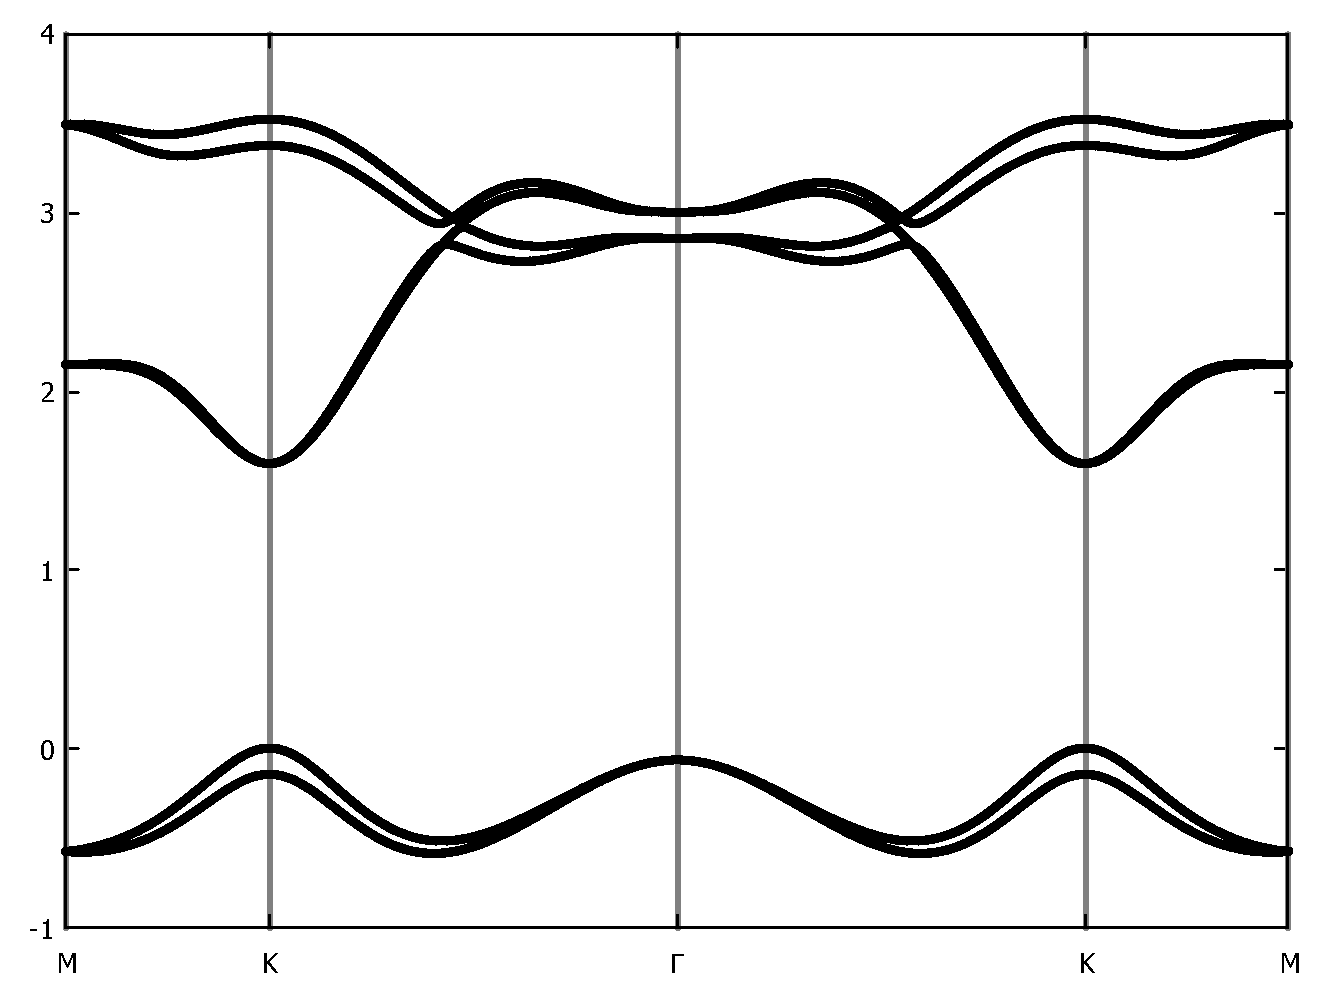
\includegraphics[width=\linewidth]{pic/bandstructureSOC.pdf}
%		%\caption{\label{band structure SOC}}
%	\end{subfigure}
%	\begin{subfigure}[b]{0.495\textwidth}
%		\centering
%		\includegraphics[width=\linewidth]{pic/bandstructureSOCTNN.pdf}
%		%\caption{\label{HB SOC}}
%	\end{subfigure}
%	\caption[Banstructure of NN and TNN monolayer MoS$_{2}$ with SOC without magnetic field.]{The band structure of monolayer MoS$_2$ in the absence of a magnetic field along the $\Gamma$–K direction exhibits significant spin splittings at the $K$ and $-K$ points, primarily due to spin–orbit coupling (SOC). Figures 2.8(a) and 2.8(b) show the results obtained using \ac{NN} and \ac{TNN} model, respectively.
%	}
%\end{figure*}
%The diagram in Fig. 2.8 shows the significant splitting of the valence bands at the $K$ and $K'$ points of MoS$_{2}$, caused by the \ac{SOC}, with a value of $\Delta_{\text{SOC}}^{\lambda} = 2 \lambda = 146$ meV. Although the \ac{NN} \ac{TB} model is not accurate as the TNN one, it can be seen that the \ac{NN} \ac{TB} bands agree well the \ac{TNN} results near the $K$ and $K'$ points.


\section{Three-band tight binding model under a magnetic field}\label{Section 3.2}
Under an uniform magnetic field given by a vector potential $\mathbf{A}(\mathbf{r})$ the single electron Hamiltonian changes into
\begin{gather}
	H = \f{\left(-i\hbar \boldsymbol{\nabla} + e \mathbf{A(r)}\right)^{2}}{2m} + U_{0}(\mathbf{r}) + g^{*} \mu_{B} \mathbf{B} \cdot \mathbf{L},
\end{gather}
where $\mu_{B} = \f{e\hbar}{2m}$ is Bohr magneton, $g^{*}$ is an effective Landé g-factor, $\mathbf{B} = \boldsymbol{\nabla} \times  \mathbf{A}$ is the uniform magnetic field, and $\mathbf{L}$ is the angular momentum. It is possible to add a phase factor to the tight-binding wavefunction
\begin{gather}
	\psi_{\lambda,\mathbf{k}} (\mathbf{r}) = \sum_{j=1}^{3} C_{j}^{\lambda}(\mathbf{k}) \sum_{\mathbf{R}} e^{i\mathbf{k \cdot R}} e^{ \theta_{\mathbf{R}}(\mathbf{r})} \phi_{j}(\mathbf{r} - \mathbf{R}).
\end{gather}
We now have
\begin{equation}
	\begin{aligned}
		H_{j j'} (\mathbf{k}) = H_{jj'}^{\text{TB}}(\mathbf{k}) + H_{jj'}^{Z}(\mathbf{k}),
	\end{aligned}
\end{equation}
where
\begin{equation}
	\begin{aligned}
		H_{jj'}^{\text{TB}}(\mathbf{k})
		& = \sum_{\mathbf{R}} \bra{\phi_{j}(\mathbf{r})} e^{-i \theta_{\mathbf{0}}(\mathbf{r})} \left[\f{(-i\hbar \boldsymbol{\nabla} + e \mathbf{A}(\mathbf{r}))^{2}}{2m} + U_{0}(\mathbf{r}) \right] e^{i\mathbf{k \cdot R}} e^{ \theta_{\mathbf{R}}(\mathbf{r})} \ket{\phi_{j'}(\mathbf{r - R})}                        \\
		& = \sum_{\mathbf{R}} \bra{\phi_{j}(\mathbf{r})} e^{i(\mathbf{k \cdot R} +\theta_{\mathbf{R}} - \theta_{\mathbf{0}} )} \left[ \f{ \left( -i\hbar \boldsymbol{\nabla} + e \mathbf{A} + \hbar \boldsymbol{\nabla} \theta_{\mathbf{R}} \right)^{2} }{2m} + U_{0}(\mathbf{r}) \right] \ket{\phi_{j'}(\mathbf{r - R})}.
	\end{aligned}
\end{equation}
Since the Zeeman interaction orginates from the coupling between the magnetic field and the orbital angular momentum of electrons localized at atomic sites, it is an on-site effect rather than a hopping term. Therefore, the Hamiltonian Zeeman is approximated by keeping only $\mathbf{R} = 0$ contribution
\begin{equation}
	\begin{aligned}
		H_{jj'}^{Z}(\mathbf{k})
		& = g^{*} \mu_{B} \mathbf{B} \cdot \sum_{\mathbf{R}} \bra{\phi_{j}(\mathbf{r})} e^{i(\mathbf{k \cdot R} + \theta_{\mathbf{R}} - \theta_{\mathbf{0}} )} \mathbf{L} \ket{\phi_{j'}(\mathbf{r - R})} \\
		& \approx g^{*} \mu_{B} \mathbf{B} \cdot \sum_{\mathbf{R}} \bra{\phi_{j}(\mathbf{r})} \mathbf{L} \ket{\phi_{j'}(\mathbf{r})}.
	\end{aligned}
\end{equation}
By choosing $\theta_{\mathbf{R}} = - \f{e}{\hbar} \int_{\mathbf{R}}^{\mathbf{r}} \mathbf{A(\mathbf{r'})} \cdot d\mathbf{r'}$ as Peierls substitution \cite{peierls1933theorie}, the Hamiltonian in Eq.~(3.20) now reads
\begin{equation}
	\begin{aligned}
		H_{jj'}^{\text{TB}}(\mathbf{k})
		& = \sum_{\mathbf{R}} \bra{\phi_{j}(\mathbf{r})} e^{i\mathbf{k \cdot R} - \frac{ie}{\hbar} \int_{\mathbf{R}}^{\mathbf{r}} \mathbf{A}(\mathbf{r'}) \cdot d\mathbf{r'} + \frac{ie}{\hbar}\int_{\mathbf{0}}^{\mathbf{r}}\mathbf{A(\mathbf{r'})}\cdot d\mathbf{r'} } \left[- \f{\hbar^{2} \boldsymbol{\nabla}^{2}}{2m} + U_{0} (\mathbf{r}) \right] \ket{\phi_{j'}(\mathbf{r - R})} \\
		& = \sum_{\mathbf{R}}  e^{i\mathbf{k \cdot R}} e^{\frac{ie}{\hbar} \int_{\mathbf{0}}^{\mathbf{R}} \mathbf{A(\mathbf{r'})} \cdot d \mathbf{r'} } \bra{\phi_{j}(\mathbf{r})} e^{-\frac{ie}{\hbar} \Phi_{\mathbf{R,r,0}}} \left[ -\f{\hbar^{2} \boldsymbol{\nabla}^{2}}{2m} + U_{0} (\mathbf{r}) \right] \ket{\phi_{j'}(\mathbf{r - R})},
	\end{aligned}
\end{equation}
where $\Phi_{\mathbf{R,r,0}} = \oint_{\mathbf{R,r,0}} \mathbf{A(\mathbf{r'})} \cdot d\mathbf{r'} $ is the closed loop line integral of $\mathbf{A}$ along the triangle points $\mathbf{R,r,0}$, and $\int_{\mathbf{0}}^{\mathbf{R}} \mathbf{A(\mathbf{r'})} \cdot d \mathbf{r'}$ is the path integral along the two points $\mathbf{R,0}$. Besides that, we have used the fact that
\begin{align}
	\int_{\mathbf{R}}^{\mathbf{r}} \mathbf{A(\mathbf{r'})} \cdot d\mathbf{r'} + \int_{\mathbf{r}}^{\mathbf{0}} \mathbf{A(r')} \cdot d\mathbf{r'} = \Phi_{\mathbf{R,r,0}} - \int_{\mathbf{0}}^{\mathbf{R}} \mathbf{A(\mathbf{r'})} \cdot d \mathbf{r'}.
\end{align}
We can show that the flux term $\Phi_{\mathbf{R}, \mathbf{r}, \mathbf{0}}$ is negligibly small based on two observations~\cite{yalcin_2019}. Firstly, when $\mathbf{r}$ is far from the lattice points $\mathbf{R}$ and $\mathbf{0}$, the enclosed flux may be large. However, since the atomic orbitals are highly localized at these two lattice sites, the corresponding hopping amplitude becomes vanishingly small, effectively suppressing the entire hopping term. Second, when $\mathbf{r}$ is located at or near either of the two lattice points, the triangle formed is small. Under the assumption of a weak magnetic field, the flux term $\Phi_{\mathbf{R}, \mathbf{r}, \mathbf{0}}$ in this case approaches zero. These considerations give us the Hamiltonian as
\begin{gather}
	H_{jj'}^{\text{TB}}(\mathbf{k})
	= \sum_{\mathbf{R}} e^{i\mathbf{k \cdot R}}e^{\frac{ie}{\hbar} \int_{\mathbf{0}}^{\mathbf{R}} \mathbf{A(\mathbf{r'})} \cdot d \mathbf{r'} } \bra{\phi_{j}(\mathbf{r})} \left[ -\f{\hbar^{2} \boldsymbol{\nabla}^{2}}{2m} + U_{0} (\mathbf{r}) \right] \ket{\phi_{j'}(\mathbf{r - R})}.
\end{gather}
Considering only \ac{NN}, \ac{NNN}, \ac{TNN} hoppings, Eq.~(3.24) becomes
\begin{equation}
	\begin{aligned}
		H_{jj'}^{\text{TB}}(\mathbf{k})
		& = \sum_{\mathbf{R}} e^{i\mathbf{k\cdot R}} e^{\frac{e}{\hbar}\int_{0}^{\mathbf{R}}A(\mathbf{r'})d\mathbf{r'}} \mathcal{E}_{jj'}(\mathbf{R})                                                                                                                                                                                                \\
		& = \mathcal{E}_{jj'}(\mathbf{0}) + e^{i\mathbf{k\cdot}\mathbf{R}_{1} }e^{\frac{e}{\hbar}\int_{0}^{\mathbf{R}_{1}}A(\mathbf{r'})d\mathbf{r'}} \mathcal{E}_{jj'}(\mathbf{R}_{1})  + e^{i\mathbf{k\cdot}\mathbf{R}_{2} }e^{\frac{e}{\hbar}\int_{0}^{\mathbf{R}_{2}}A(\mathbf{r'})d\mathbf{r'}} \mathcal{E}_{jj'}(\mathbf{R}_{2})               \\
		& + e^{i\mathbf{k\cdot}\mathbf{R}_{3} }e^{\frac{e}{\hbar}\int_{0}^{\mathbf{R}_{3}}A(\mathbf{r'})d\mathbf{r'}} \mathcal{E}_{jj'}(\mathbf{R}_{3})+ e^{i\mathbf{k\cdot}\mathbf{R}_{4} }e^{\frac{e}{\hbar}\int_{0}^{\mathbf{R}_{4}}A(\mathbf{r'})d\mathbf{r'}} \mathcal{E}_{jj'}(\mathbf{R}_{4})                                                 \\
		& + e^{i\mathbf{k\cdot}\mathbf{R}_{5} }e^{\frac{e}{\hbar}\int_{0}^{\mathbf{R}_{5}}A(\mathbf{r'})d\mathbf{r'}} \mathcal{E}_{jj'}(\mathbf{R}_{5})+ e^{i\mathbf{k\cdot}\mathbf{R}_{6} }e^{\frac{e}{\hbar}\int_{0}^{\mathbf{R}_{6}}A(\mathbf{r'})d\mathbf{r'}} \mathcal{E}_{jj'}(\mathbf{R}_{6})                                                 \\
		& + e^{i\mathbf{k\cdot}\tilde{\mathbf{R}}_{1} }e^{\frac{e}{\hbar}\int_{0}^{\tilde{\mathbf{R}}_{1}}A(\mathbf{r'})d\mathbf{r'}} \mathcal{E}_{jj'}(\tilde{\mathbf{R}}_{1})+ e^{i\mathbf{k\cdot}\tilde{\mathbf{R}}_{2} }e^{\frac{e}{\hbar}\int_{0}^{\tilde{\mathbf{R}}_{2}}A(\mathbf{r'})d\mathbf{r'}} \mathcal{E}_{jj'}(\tilde{\mathbf{R}}_{2}) \\
		& + e^{i\mathbf{k\cdot}\tilde{\mathbf{R}}_{3} }e^{\frac{e}{\hbar}\int_{0}^{\tilde{\mathbf{R}}_{3}}A(\mathbf{r'})d\mathbf{r'}} \mathcal{E}_{jj'}(\tilde{\mathbf{R}}_{3})+ e^{i\mathbf{k\cdot}\tilde{\mathbf{R}}_{4} }e^{\frac{e}{\hbar}\int_{0}^{\tilde{\mathbf{R}}_{4}}A(\mathbf{r'})d\mathbf{r'}} \mathcal{E}_{jj'}(\tilde{\mathbf{R}}_{4}) \\
		& + e^{i\mathbf{k\cdot}\tilde{\mathbf{R}}_{5} }e^{\frac{e}{\hbar}\int_{0}^{\tilde{\mathbf{R}}_{5}}A(\mathbf{r'})d\mathbf{r'}} \mathcal{E}_{jj'}(\tilde{\mathbf{R}}_{5})+ e^{i\mathbf{k\cdot}\tilde{\mathbf{R}}_{6} }e^{\frac{e}{\hbar}\int_{0}^{\tilde{\mathbf{R}}_{6}}A(\mathbf{r'})d\mathbf{r'}} \mathcal{E}_{jj'}(\tilde{\mathbf{R}}_{6}) \\
		& + e^{i\mathbf{k\cdot}\mathbf{R}'_{1} }e^{\frac{e}{\hbar}\int_{0}^{\mathbf{R}'_{1}}A(\mathbf{r'})d\mathbf{r'}} \mathcal{E}_{jj'}(\mathbf{R}'_{1})+ e^{i\mathbf{k\cdot}\mathbf{R}'_{2} }e^{\frac{e}{\hbar}\int_{0}^{\mathbf{R}'_{2}}A(\mathbf{r'})d\mathbf{r'}} \mathcal{E}_{jj'}(\mathbf{R}'_{2})                                                 \\
		& + e^{i\mathbf{k\cdot}\mathbf{R}'_{3} }e^{\frac{e}{\hbar}\int_{0}^{\mathbf{R}'_{3}}A(\mathbf{r'})d\mathbf{r'}} \mathcal{E}_{jj'}(\mathbf{R}'_{3})+ e^{i\mathbf{k\cdot}\mathbf{R}'_{4} }e^{\frac{e}{\hbar}\int_{0}^{\mathbf{R}'_{4}}A(\mathbf{r'})d\mathbf{r'}} \mathcal{E}_{jj'}(\mathbf{R}'_{4})                                                 \\
		& + e^{i\mathbf{k\cdot}\mathbf{R}'_{5} }e^{\frac{e}{\hbar}\int_{0}^{\mathbf{R}'_{5}}A(\mathbf{r'})d\mathbf{r'}} \mathcal{E}_{jj'}(\mathbf{R}'_{5})+ e^{i\mathbf{k\cdot}\mathbf{R}'_{6} }e^{\frac{e}{\hbar}\int_{0}^{\mathbf{R}'_{6}}A(\mathbf{r'})d\mathbf{r'}} \mathcal{E}_{jj'}(\mathbf{R}'_{6})     ,                                            \\
	\end{aligned}
\end{equation}
where $\mathbf{R}_{i}$, $\tilde{\mathbf{R}}_{i}$ and $\mathbf{R}'_{i} = 2 \mathbf{R}_{i}$ are \ac{NN}, \ac{NNN}, \ac{TNN} vectors, with $i = 1,2,...,6$.

In the presence of a perpendicular magnetic field $\mathbf{B} = (0,0,B)$ applied to the plane of \ac{TMD}, we choose the vector potential in the Landau gauge as $\mathbf{A} = (0, Bx, 0)$. Suppose that the atom metal M is located at position $\mathbf{R}_{m,n} = \left(m \frac{a}{2}, n \frac{a\sqrt{3}}{2}\right)$, where $m,n \in \mathbb{Z}$, let us define a shorthand notation for these extra terms
\begin{equation}
	\begin{aligned}
		\theta_{m,n}^{m',n'}
		& = \frac{e}{\hbar} \int_{m,n}^{m',n'} \mathbf{A}(\mathbf{r}) \cdot d\mathbf{r} \\
		& = \frac{eB}{2\hbar}(x_{m} + x_{m'})(y_{n'} - y_{n}),
	\end{aligned}
\end{equation}
Here, the nineteen hopping coordinates considered up to TNN are given by $x_{m} = \frac{ma}{2}$ ($m = \pm 1, \pm 2$) and $y_{n} = \frac{na\sqrt{3}}{2}$ ($n = 0, \pm 1$), where $a$ is the lattice constant, are shown in \hyperref[fig:site index]{Fig. 3.2}. Details of the derivation of the Eq.~(3.26) are given in \hyperref[appendix B]{Appendix B}.
\begin{figure}[H]
	\centering
	\includegraphics[width=0.85\linewidth]{pic/siteindex_2_crop.pdf}
	\caption[TMD with eighteen neighbors atom M rewrite with the site index.]{\label{fig:site index} The \ac{TBM} of \ac{TMD} with eighteen neighbor atoms M rewrite with the site index.}
\end{figure}

%In this system, hopping integral of $y$-direction does not change, but hopping integral of $y$-direction change and it depends on the $x$ position.
%Let us now express the Hamiltonian from the zero-field are given by Eq. (2.31) with the transform hopping parameters, noting that the \ac{NN} coordinates are $x = \frac{ma}{2}(m = \pm 1, \pm 2)$ and $y = \frac{na\sqrt{3}}{2}(n = 0,\pm 1)$, $a$ being the lattice constant, are shown in \hyperref[fig:site index]{Fig (2.2)}. 
\noindent Since $dy = 0$ along the $x$ direction, $\theta_{m,n}^{m \pm 2, n} = 0$, and using \ac{TNN} coordinates given for lattice site in \hyperref[Table 2.1]{Table~3.1}, the $\theta_{m,n}^{m',n'}$ can be written as
%\begin{table}[h]
%	\begin{equation*}
	%		\renewcommand{\arraystretch}{1.5}
	%		\begin{NiceArray}{c c c}
		%			\hline
		%			\hline
		%			\text{Vector}          & \text{Hopping relative coordinates} & \text{Peierls phase}\theta_{m,n}^{m',n'} \\
		%			\hline
		%			\mathbf{R}_{1}         & (m,n) \to (m+2,n)                     & a (1,0,0)                      \\
		%			\mathbf{R}_{2}         & (m,n) \to (m+1,n-1)                   & a \left(\frac{1}{2},-\frac{\sqrt{3}}{2},0\right)                      \\
		%			\mathbf{R}_{3}         & (m,n) \to (m-1,n-1)                   & a \left(-\frac{1}{2},-\frac{\sqrt{3}}{2},0\right)                      \\
		%			\mathbf{R}_{4}         & (m,n) \to (m-2,n)                     & a (-1,0,0)                      \\
		%			\mathbf{R}_{5}         & (m,n) \to (m-1,n+1)                   & a \left(-\frac{1}{2},\frac{\sqrt{3}}{2},0\right)                      \\
		%			\mathbf{R}_{6}         & (m,n) \to (m+1,n+1)                   & a \left(-\frac{1}{2},\frac{\sqrt{3}}{2},0\right)                      \\
		%			\tilde{\mathbf{R}}_{1} & (m,n) \to (m+3,n-1)                   & l \left(\frac{\sqrt{3}}{2},-\frac{1}{2},0\right)                      \\
		%			\tilde{\mathbf{R}}_{2} & (m,n) \to (m,n-2)                     & l \left(0,-1,0\right)                      \\
		%			\tilde{\mathbf{R}}_{3} & (m,n) \to (m-3,n-1)                   & l \left(-\frac{\sqrt{3}}{2},-\frac{1}{2},0\right)                      \\
		%			\tilde{\mathbf{R}}_{4} & (m,n) \to (m-3,n+1)                   & l \left(-\frac{\sqrt{3}}{2},\frac{1}{2},0\right)                      \\
		%			\tilde{\mathbf{R}}_{5} & (m,n) \to (m,n+2)                     & l \left(0,-1,0\right)                      \\
		%			\tilde{\mathbf{R}}_{6} & (m,n) \to (m+3,n+1)                   & l \left(\frac{\sqrt{3}}{2},\frac{1}{2},0\right)                      \\
		%			2\mathbf{R}_{1}        & (m,n) \to (m+4,n)                     & a (2,0,0)                      \\
		%			2\mathbf{R}_{2}        & (m,n) \to (m+2,n-2)                   & a (1,-\sqrt{3},0)                      \\
		%			2\mathbf{R}_{3}        & (m,n) \to (m-2,n-2)                   & a (-1,-\sqrt{3},0)                      \\
		%			2\mathbf{R}_{4}        & (m,n) \to (m-4,n)                     & a (-2,0,0)                      \\
		%			2\mathbf{R}_{5}        & (m,n) \to (m-2,n+2)                   & a (-1,\sqrt{3},0)                      \\
		%			2\mathbf{R}_{6}        & (m,n) \to (m+2,n+2)                   & a (1,\sqrt{3},0)                      \\
		%			\hline 
		%			\hline
		%		\end{NiceArray}
	%	\end{equation*}
%	\caption[Peierls phase.]{Caption.}
%\end{table}
\begin{gather}
	\theta_{m,n}^{m',n'} =
	\begin{cases}
		0                                                                             & \quad m' = m \pm 2, n' = n  ,      \\
		0                                                                             & \quad m' = m \pm 4, n' = n  ,      \\
		\pm \frac{e}{\hbar} \frac{B a^{2} \sqrt{3}}{2} m                      & \quad m' = m , n' = n \pm 2,  \\
		\pm \frac{e}{\hbar} \frac{B a^{2} \sqrt{3}}{4} \left(m \mp \frac{1}{2}\right) & \quad m' = m \mp 1, n' = n \pm 1 , \\
		\pm \frac{e}{\hbar} \frac{B a^{2} \sqrt{3}}{2} (m \mp 1)                      & \quad m' = m \mp 2, n' = n \pm 2,  \\
		\pm \frac{e}{\hbar} \frac{B a^{2} \sqrt{3}}{4} \left(m \mp \frac{3}{2}\right) & \quad m' = m \mp 3, n' = n \pm 1.  \\
	\end{cases}
\end{gather}
Identifying $\frac{B a^{2} \sqrt{3}}{2}$ as the magnetic flux $\Phi$ passing through per unit cell and $\frac{h}{e}$ corresponds to the magnetic flux quantum $\Phi_{0}$, we obtain the following relation
\begin{equation}
	\begin{aligned}
		H_{jj'}(\mathbf{k})
		& = \mathcal{E}_{jj'}(\mathbf{0}) + e^{i \mathbf{k} \cdot \mathbf{R}_{1}} \mathcal{E}_{jj'}(\mathbf{R}_{1}) + e^{-i\pi(m + 1/2)\Phi / \Phi_{0}} e^{i \mathbf{k} \cdot \mathbf{R}_{2}} \mathcal{E}_{jj'}(\mathbf{R}_{2})  \\
		& + e^{-i\pi(m - 1/2)\Phi / \Phi_{0}} e^{i \mathbf{k} \cdot \mathbf{R}_{3}} \mathcal{E}_{jj'}(\mathbf{R}_{3}) + e^{i \mathbf{k} \cdot \mathbf{R}_{4}} \mathcal{E}_{jj'}(\mathbf{R}_{4})                                  \\
		& + e^{i\pi(m - 1/2)\Phi / \Phi_{0}} e^{i \mathbf{k} \cdot \mathbf{R}_{5}} \mathcal{E}_{jj'}(\mathbf{R}_{5}) + e^{i\pi(m + 1/2)\Phi / \Phi_{0}} e^{i \mathbf{k} \cdot \mathbf{R}_{6}} \mathcal{E}_{jj'}(\mathbf{R}_{6}) \\
		& + e^{- i\pi(m + 3/2)\Phi/\Phi_{0} } e^{i \mathbf{k} \cdot \tilde{\mathbf{R}}_{1}} \mathcal{E}_{jj'}(\tilde{\mathbf{R}}_{1}) + e^{- 2i\pi m\Phi/\Phi_{0} } e^{i \mathbf{k} \cdot \tilde{\mathbf{R}}_{2}} \mathcal{E}_{jj'}(\tilde{\mathbf{R}}_{2}) \\
		& + e^{- i\pi(m - 3/2)\Phi/\Phi_{0} } e^{i \mathbf{k} \cdot \tilde{\mathbf{R}}_{3}} \mathcal{E}_{jj'}(\tilde{\mathbf{R}}_{3}) + e^{ i\pi (m-3/2)\Phi/\Phi_{0} } e^{i \mathbf{k} \cdot \tilde{\mathbf{R}}_{4}} \mathcal{E}_{jj'}(\tilde{\mathbf{R}}_{4}) \\
		& + e^{2 i\pi m \Phi/\Phi_{0} } e^{i \mathbf{k} \cdot \tilde{\mathbf{R}}_{5}} \mathcal{E}_{jj'}(\tilde{\mathbf{R}}_{5}) + e^{ i\pi (m+3/2)\Phi/\Phi_{0} } e^{i \mathbf{k} \cdot \tilde{\mathbf{R}}_{6}} \mathcal{E}_{jj'}(\tilde{\mathbf{R}}_{6}) \\
		& + e^{i \mathbf{k} \cdot \mathbf{R}'_{1}} \mathcal{E}_{jj'}(\mathbf{R}'_{1}) + e^{-2i\pi(m + 1)\Phi / \Phi_{0}} e^{i \mathbf{k} \cdot \mathbf{R}'_{2}} \mathcal{E}_{jj'}(\mathbf{R}'_{2})  \\
		& + e^{-2i\pi(m - 1)\Phi / \Phi_{0}} e^{i \mathbf{k} \cdot \mathbf{R}'_{3}} \mathcal{E}_{jj'}(\mathbf{R}'_{3}) + e^{i \mathbf{k} \cdot \mathbf{R}'_{4}} \mathcal{E}_{jj'}(\mathbf{R}'_{4})                                  \\
		& + e^{2i\pi(m - 1)\Phi / \Phi_{0}} e^{i \mathbf{k} \cdot \mathbf{R}'_{5}} \mathcal{E}_{jj'}(\mathbf{R}'_{5}) + e^{2i\pi(m + 1)\Phi / \Phi_{0}} e^{i \mathbf{k} \cdot \mathbf{R}'_{6}} \mathcal{E}_{jj'}(\mathbf{R}'_{6}).
	\end{aligned}
\end{equation}

The Hamiltonian matrix element in Eq.~(3.28) depends only on the site index $m$ and does not invariant under the expansion of a lattice vector along the $x$ axis. In order to restore this invariance, we can look at the case where the ratio of magnetic flux and flux quanta is a rational number $\Phi / \Phi_{0} = p / q$. The crucial advantage of the Peierls phase approach is that it allows the lattice periodicity to be restored, provided that a suitable magnetic unit cell or ``magnetic supercell'' containing several original unit cells is constructed. One might ask what truly happens inside the magnetic unit cells. Do the neighbor interactions remain the same way as they did in the tight-binding model? We will explore this after deriving the Hamiltonian for the magnetic unit cell.

%The magnetic unit cell has lattice vectors $q\mathbf{a}_{1}$ and $\mathbf{a}_{2}$ are illustrated in Fig. (2.5)
\begin{figure}[H]
	\centering
	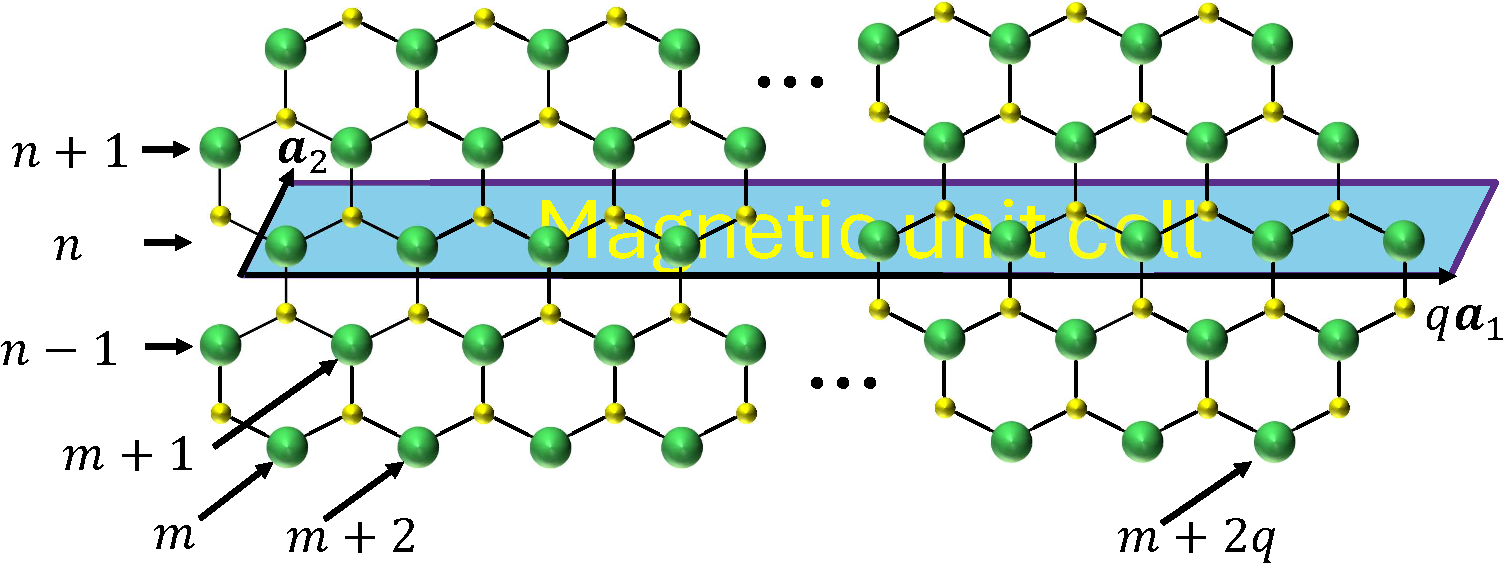
\includegraphics[width=\linewidth]{pic/magneticUC_cut.pdf}
	\caption[Magnetic unit cell for TMD monolayers.]{\label{fig:Mag UC}Magnetic unit cell for TMD monolayers.}
\end{figure}
%Hinh. 

In Section~3.1, we ignored the sum over of relative positions $\mathbf{r}_{i}$ in Eq.~(2.3) as the orbitals of X atoms were neglected. However, the magnetic unit cell consits $2q$ atom M. We now define a new basis set of $6q$ atomic orbitals $\{ \phi_{j}(\mathbf{r} - \mathbf{r}_{i}) \}$ where $j=1,2,3$ and $\mathbf{r}_{i} \in \text{MUC}$.
%Here, $\mathbf{r}_{i} = (x_{i},y_{i}) = \frac{ma}{2}\hat{x} + \frac{na\sqrt{3}}{2}\hat{y}$. 
The new basis function now is
\begin{gather}
	\psi_{\lambda,\mathbf{k}}(\mathbf{r}) = \sum_{j}^{3}\sum_{i}^{2q} C_{ji}^{\lambda}(\mathbf{k}) \sum_{{\alpha}} e^{i\mathbf{k}\cdot(\mathbf{R}_{\alpha} + \mathbf{r}_{i})} \phi_{j}(\mathbf{r} - \mathbf{R}_{\alpha} - \mathbf{r}_{i}).
\end{gather}
Here, we set $\mathbf{r}_{i}$ refers to the position of an atom in a unit cell, while $\mathbf{R}_{\alpha}$ denotes the position of different unit cells.
The Hamiltonian matrix elements in the new basis is written as
\begin{equation}
	\begin{aligned}
		H_{jj'}^{ii'}(\mathbf{k})
		&= \sum_{{\alpha}}\sum_{{\beta}} e^{i \mathbf{k} \cdot (\mathbf{R}_{\beta} - \mathbf{R}_{\alpha} + \mathbf{r}_{i'} - \mathbf{r}_{i})}  \bra{\phi_{j}(\mathbf{r} - \mathbf{R}_{\alpha} - \mathbf{r}_{i})} \left[-\tfrac{\hbar^{2} \boldsymbol{\nabla}^{2}}{2m} + U_{0}\right] \ket{\phi_{j}(\mathbf{r} - \mathbf{R}_{\beta} - \mathbf{r}_{i'})} \\
		&=\sum_{{\alpha}}\sum_{{\beta}} e^{i \mathbf{k} \cdot (\mathbf{R}_{\beta} - \mathbf{R}_{\alpha} + \mathbf{r}_{m',n'} - \mathbf{r}_{m,n})}  \bra{\phi_{j}(\mathbf{r} - \mathbf{R}_{\alpha} - \mathbf{r}_{m,n})} \left[-\tfrac{\hbar^{2} \boldsymbol{\nabla}^{2}}{2m} + U_{0}\right] \ket{\phi_{j}(\mathbf{r} - \mathbf{R}_{\beta} - \mathbf{r}_{m',n'})} .
	\end{aligned}
\end{equation}
Now we center our system at $\mathbf{r}'=\mathbf{r} - \mathbf{R}_{\alpha} - \mathbf{r}_{m,n}$ and define $\mathbf{R}_{\gamma} = \mathbf{R}_{\alpha} - \mathbf{R}_{\beta}$. We get
\begin{gather}
	H_{jj'}^{ii'}(\mathbf{k})
	= \sum_{{\alpha}}\sum_{{\gamma}} e^{-i \mathbf{k} \cdot (\mathbf{R}_{\gamma} + \mathbf{r}_{m,n} - \mathbf{r}_{m',n'})}  \bra{\phi_{j}(\mathbf{r})} \left[-\tfrac{\hbar^{2} \boldsymbol{\nabla}^{2}}{2m} + U_{0}\right] \ket{\phi_{j}(\mathbf{r} + \mathbf{R}_{\gamma} + \mathbf{r}_{m,n} - \mathbf{r}_{m',n'})}.
\end{gather}
Taking the sum over $\mathbf{R}_{\gamma}$ considering only \ac{NN}, \ac{NNN}, \ac{TNN} such that $\abs{\mathbf{R}_{\gamma}} \leq a$. The lattice vectors that satisfying this condition is $\mathbf{R}_{\gamma} = 0$. 
%We can choose $\mathbf{R}_{\alpha} = \mathbf{0}$, this will not affect the Hamiltonian. In fact, the sum over $\mathbf{R}$ is only considering the \ac{NN}, \ac{NNN}, \ac{TNN} atoms, and replacing $\mathbf{R}$ is equivalent to redefining dummy variables in the equation.
%and replacing $\mathbf{r}_{i} = \left(m \frac{a}{2}, n \frac{a\sqrt{3}}{2}\right)$, $\mathbf{r}_{i'} = \left(m' \frac{a}{2}, n' \frac{a\sqrt{3}}{2}\right)$, notice that $i = (m,n)$ 
Since only the \ac{NN}, \ac{NNN} and \ac{TNN} are considered, the matrix elements $\bra{\phi_{j}(\mathbf{r})} \left[-\tfrac{\hbar^{2} \boldsymbol{\nabla}^{2}}{2m} + U_{0}\right] \ket{\phi_{j}(\mathbf{r} + \mathbf{r}_{m,n} - \mathbf{r}_{m',n'})}$ are nonzero when $\mathbf{r}_{m',n'} = \mathbf{r}_{m,n} + \mathbf{R}$, where $\mathbf{R} = 0$ or a displacement vector connecting to a \ac{NN}, \ac{NNN}, \ac{TNN} atoms, the Hamiltonian matrix elemtents are written in the form

\begin{gather}
	H_{jj'}^{ii'}(\mathbf{k}) =\sum_{\mathbf{R}} e^{i \mathbf{k}\cdot \mathbf{R}} \bra{\phi_{j}(\mathbf{r})} \left[-\f{\hbar^{2} \boldsymbol{\nabla}^{2}}{2m} + U_{0}(\mathbf{r})\right] \ket{\phi_{j'}(\mathbf{r}-\mathbf{R})}\delta_{m + \Delta m_{\mathbf{R}},m'} \delta_{n + \Delta n_{\mathbf{R}},n'},
\end{gather}
here ($\Delta m_{\mathbf{R}}, \Delta n_{\mathbf{R}}$) the hopping relative coordinates are given in \hyperref[Table 2.1]{Table 3.1}. 
%, we define our hopping terms in the new basis is given by
%\begin{gather}
%	H_{jj'}^{ii'}(\mathbf{k}) = \sum_{{\alpha}}\sum_{{\gamma}} e^{-i \mathbf{k}\cdot \mathbf{R}_{\gamma}} \bra{\phi_{j}(\mathbf{r})} \left[-\f{\hbar^{2} \boldsymbol{\nabla}^{2}}{2m} + U_{0}(\mathbf{r})\right] \ket{\phi_{j'}(\mathbf{r}+\mathbf{R}_{\gamma})}\delta_{i,i'}.
%\end{gather}

One can regconize that Eq.~(3.32) resembles Eq.~(3.4). Additionally, the equation not only describes the hopping between magnetic unit cells but also accounts for hopping between sites within magnetic unit cells. To address the previous question, it is important to note that we have enlarged the original unit cell into a magnetic unit cell, which now contains $2q$ atoms M. The neighbor interactions are preserved inside the ``supercell'', but they now involve neighboring magnetic unit cells due to the enlarged cell structure. The Hamiltonian has a discrete tranlastional invariance with a unit cell carrying $2q$ unit cells along the $x$ axis.

%The last step is to develop the matrix Hamiltonian elements. This can be obtained by taking the sum over $\mathbf{R}$ in Eq. (2.31). We can choose $\mathbf{R}_{\alpha} = \mathbf{0}$, this will not affect the Hamiltonian. In fact, the sum over $\mathbf{R}$ is only considering the \ac{NN}, \ac{NNN}, \ac{TNN} atoms, and replacing $\mathbf{R}$ is equivalent to redefining dummy variables in the equation, 
The Hamiltonian with the Peierls phase now is
\begin{gather}
	H_{jj'}^{ii'}(\mathbf{k}) =\sum_{\mathbf{R}} e^{i \theta_{m,n}^{m + \Delta m_{\mathbf{R}},n + \Delta n_{\mathbf{R}}} } e^{i \mathbf{k}\cdot \mathbf{R}} \bra{\phi_{j}(\mathbf{r})} \left[-\tfrac{\hbar^{2} \boldsymbol{\nabla}^{2}}{2m} + U_{0}(\mathbf{r})\right] \ket{\phi_{j'}(\mathbf{r}-\mathbf{R})}\delta_{m + \Delta m_{\mathbf{R}},m'} \delta_{n + \Delta n_{\mathbf{R}},n'}.
\end{gather}
%\begin{equation}
%	\begin{aligned}
	%		& H_{jmnj'm'n'}(\mathbf{k})
	%		= e^{i\theta_{m,n}^{m,n}}e^{i\mathbf{k} \cdot (\mathbf{0} - \mathbf{0})} \bra{\phi_{j}(\mathbf{r})} H_{0} \ket{\phi_{j'}(\mathbf{r})}\delta_{m,m'}^{n,n'}                             
	%		 + e^{i\theta_{m,n}^{m+2,n}}e^{i\mathbf{k} \cdot (\mathbf{R}_{1} - \mathbf{0})} \bra{\phi_{j}(\mathbf{r})} H_{0} \ket{\phi_{j'}(\mathbf{r}-\mathbf{R}_{1})}\delta_{m+2,m}^{n,n'}     \\
	%		& + e^{i\theta_{m,n}^{m-2,n}}e^{i\mathbf{k} \cdot (\mathbf{R}_{4} - \mathbf{0})} \bra{\phi_{j}(\mathbf{r})} H_{0} \ket{\phi_{j'}(\mathbf{r}-\mathbf{R}_{4})}\delta_{m-2,m'}^{n,n'}    \\
	%		& + e^{i\theta_{m,n}^{m+1,n-1}}e^{i\mathbf{k} \cdot (\mathbf{R}_{2} - \mathbf{0})} \bra{\phi_{j}(\mathbf{r})} H_{0} \ket{\phi_{j'}(\mathbf{r}-\mathbf{R}_{2})}\delta_{m+1,m}^{n-1,n'} \\
	%		& + e^{i\theta_{m,n}^{m-1,n-1}}e^{i\mathbf{k} \cdot (\mathbf{R}_{3}-\mathbf{0})} \bra{\phi_{j}(\mathbf{r})} H_{0} \ket{\phi_{j'}(\mathbf{r}-\mathbf{R}_{3})}\delta_{m-1,m'}^{n-1,n'}  \\
	%		& + e^{i\theta_{m,n}^{m-1,n+1}}e^{i\mathbf{k} \cdot (\mathbf{R}_{5}-\mathbf{0})} \bra{\phi_{j}(\mathbf{r})} H_{0} \ket{\phi_{j'}(\mathbf{r}-\mathbf{R}_{5})}\delta_{m-1,m'}^{n+1,n'}  \\
	%		& + e^{i\theta_{m,n}^{m+1,n+1}}e^{i\mathbf{k} \cdot (\mathbf{R}_{6}-\mathbf{0})} \bra{\phi_{j}(\mathbf{r})} H_{0} \ket{\phi_{j'}(\mathbf{r}-\mathbf{R}_{6})}\delta_{m+1,m'}^{n+1,n'} \\
	%		& + e^{i\theta_{m,n}^{m+3,n-1}}e^{i\mathbf{k} \cdot (\tilde{\mathbf{R}}_{1}-\mathbf{0})} \bra{\phi_{j}(\mathbf{r})} H_{0} \ket{\phi_{j'}(\mathbf{r}-\tilde{\mathbf{R}}_{1})}\delta_{m+3,m'}^{n-1,n'} \\
	%		& + e^{i\theta_{m,n}^{m,n-2}}e^{i\mathbf{k} \cdot (\tilde{\mathbf{R}}_{2}-\mathbf{0})} \bra{\phi_{j}(\mathbf{r})} H_{0} \ket{\phi_{j'}(\mathbf{r}-\tilde{\mathbf{R}}_{2})}\delta_{m,m'}^{n-2,n'} \\
	%		& + e^{i\theta_{m,n}^{m-3,n-1}}e^{i\mathbf{k} \cdot (\tilde{\mathbf{R}}_{3}-\mathbf{0})} \bra{\phi_{j}(\mathbf{r})} H_{0} \ket{\phi_{j'}(\mathbf{r}-\tilde{\mathbf{R}}_{3})}\delta_{m-3,m'}^{n-1,n'} \\
	%		& + e^{i\theta_{m,n}^{m-3,n+1}}e^{i\mathbf{k} \cdot (\tilde{\mathbf{R}}_{4}-\mathbf{0})} \bra{\phi_{j}(\mathbf{r})} H_{0} \ket{\phi_{j'}(\mathbf{r}-\tilde{\mathbf{R}}_{4})}\delta_{m-3,m'}^{n+1,n'} \\
	%		& + e^{i\theta_{m,n}^{m,n+2}}e^{i\mathbf{k} \cdot (\tilde{\mathbf{R}}_{5}-\mathbf{0})} \bra{\phi_{j}(\mathbf{r})} H_{0} \ket{\phi_{j'}(\mathbf{r}-\tilde{\mathbf{R}}_{5})}\delta_{m,m'}^{n+2,n'} \\
	%		& + e^{i\theta_{m,n}^{m+3,n+1}}e^{i\mathbf{k} \cdot (\tilde{\mathbf{R}}_{6}-\mathbf{0})} \bra{\phi_{j}(\mathbf{r})} H_{0} \ket{\phi_{j'}(\mathbf{r}-\tilde{\mathbf{R}}_{6})}\delta_{m+3,m'}^{n+1,n'} \\
	%		& + e^{i\theta_{m,n}^{m+4,n}}e^{i\mathbf{k} \cdot (\mathbf{R}'_{1} - \mathbf{0})} \bra{\phi_{j}(\mathbf{r})} H_{0} \ket{\phi_{j'}(\mathbf{r}-\mathbf{R}'_{1})}\delta_{m+2,m}^{n,n'}     \\
	%		& + e^{i\theta_{m,n}^{m-4,n}}e^{i\mathbf{k} \cdot (\mathbf{R}'_{4} - \mathbf{0})} \bra{\phi_{j}(\mathbf{r})} H_{0} \ket{\phi_{j'}(\mathbf{r}-\mathbf{R}'_{4})}\delta_{m-2,m'}^{n,n'}    \\
	%		& + e^{i\theta_{m,n}^{m+2,n-2}}e^{i\mathbf{k} \cdot (\mathbf{R}'_{2} - \mathbf{0})} \bra{\phi_{j}(\mathbf{r})} H_{0} \ket{\phi_{j'}(\mathbf{r}-\mathbf{R}'_{2})}\delta_{m+1,m}^{n-1,n'} \\
	%		& + e^{i\theta_{m,n}^{m-2,n-2}}e^{i\mathbf{k} \cdot (\mathbf{R}'_{3}-\mathbf{0})} \bra{\phi_{j}(\mathbf{r})} H_{0} \ket{\phi_{j'}(\mathbf{r}-\mathbf{R}'_{3})}\delta_{m-1,m'}^{n-1,n'}  \\
	%		& + e^{i\theta_{m,n}^{m-2,n+2}}e^{i\mathbf{k} \cdot (\mathbf{R}'_{5}-\mathbf{0})} \bra{\phi_{j}(\mathbf{r})} H_{0} \ket{\phi_{j'}(\mathbf{r}-\mathbf{R}'_{5})}\delta_{m-1,m'}^{n+1,n'}  \\
	%		& + e^{i\theta_{m,n}^{m+2,n+2}}e^{i\mathbf{k} \cdot (\mathbf{R}'_{6}-\mathbf{0})} \bra{\phi_{j}(\mathbf{r})} H_{0} \ket{\phi_{j'}(\mathbf{r}-\mathbf{R}'_{6})}\delta_{m+1,m'}^{n+1,n'}, \\
	%	\end{aligned}
%\end{equation}
Simplizing Eq.~(3.33), we get the Hamiltonian for the magnetic unit cell
%\begin{equation}
%	\begin{aligned}
	%		& H_{ii'}^{jj'}(\mathbf{k})
	%		= \bra{\phi_{j}(\mathbf{r},m,n)} \left[-\tfrac{\hbar^{2}\nabla^{2}}{2m} + U_{0}\right] \ket{\phi_{j}(\mathbf{r},\mathbf{0},m,n)} \delta_{m,m}\delta_{n,n}                                                                                            \\
	%		+ & e^{-2i\alpha} e^{i\theta_{m,n}^{m+2,n}} \bra{\phi_{j}(\mathbf{r},m,n)} \left[-\tfrac{\hbar^{2}\nabla^{2}}{2m} + U_{0}\right] \ket{\phi_{j}(\mathbf{r},\mathbf{R}_{1},m,n)}\delta_{m+2,m}\delta_{n,n}                              \\
	%		+ & e^{2i\alpha} e^{i\theta_{m,n}^{m-2,n}} \bra{\phi_{j}(\mathbf{r},m,n)} \left[-\tfrac{\hbar^{2}\nabla^{2}}{2m} + U_{0}\right] \ket{\phi_{j}(\mathbf{r},\mathbf{R}_{4},m-2,n)}  \delta_{m-2,m}\delta_{n,n}                          \\
	%		+ & e^{i(\alpha - \beta)} e^{i\theta_{m,n}^{m+1,n-1}} \bra{\phi_{j}(\mathbf{r},m,n)} \left[-\tfrac{\hbar^{2}\nabla^{2}}{2m} + U_{0}\right] \ket{\phi_{j}(\mathbf{r},\mathbf{R}_{2},m+1,n-1)}                       \\
	%		+ & e^{i(-\alpha - \beta)} e^{i\theta_{m,n}^{m-1,n-1}} \bra{\phi_{j}(\mathbf{r},m,n)} \left[-\tfrac{\hbar^{2}\nabla^{2}}{2m} + U_{0}\right] \ket{\phi_{j}(\mathbf{r},\mathbf{R}_{3},m-1,n-1)}     \\
	%		+ & e^{i(-\alpha + \beta)} e^{i\theta_{m,n}^{m-1,n+1}} \bra{\phi_{j}(\mathbf{r},m,n)} \left[-\tfrac{\hbar^{2}\nabla^{2}}{2m} + U_{0}\right] \ket{\phi_{j}(\mathbf{r},\mathbf{R}_{5},m-1,n+1)}                       \\
	%		+ & e^{i(\alpha + \beta)} e^{i\theta_{m,n}^{m+1,n+1}} \bra{\phi_{j}(\mathbf{r},m,n)} \left[-\tfrac{\hbar^{2}\nabla^{2}}{2m} + U_{0}\right] \ket{\phi_{j}(\mathbf{r},\mathbf{R}_{6},m+1,n+1)}  . \\
	%	\end{aligned}
%\end{equation}
%\begin{equation}
%	\begin{aligned}
	%		& H_{ii'}^{jj'}(\mathbf{k})
	%		= \bra{\phi_{j}(\mathbf{r} -  m \mathbf{a}_{1} - n\mathbf{a}_{2})} \left[-\frac{\hbar^{2}\nabla^{2}}{2m} + U_{0}\right] \ket{\phi_{j}(\mathbf{r} -  m \mathbf{a}_{1} - n\mathbf{a}_{2})} \delta_{m,m'}^{n,n'}                                                                                                \\
	%		+ & e^{i\mathbf{k}\cdot\mathbf{a}_{1}} e^{i\theta_{m,n}^{m',n'}} \bra{\phi_{j}(\mathbf{r} - m \mathbf{a}_{1} - n\mathbf{a}_{2})} \left[-\frac{\hbar^{2}\nabla^{2}}{2m} + U_{0}\right] \ket{\phi_{j}(\mathbf{r} - (m+2) \mathbf{a}_{1} - n\mathbf{a}_{2})} \delta_{m+2,m'}^{n,n'}                             \\
	%		+ & e^{-i\mathbf{k}\cdot\mathbf{a}_{1}} e^{i\theta_{m,n}^{m',n'}} \bra{\phi_{j}(\mathbf{r} - m \mathbf{a}_{1} - n\mathbf{a}_{2})} \left[-\frac{\hbar^{2}\nabla^{2}}{2m} + U_{0}\right] \ket{\phi_{j}(\mathbf{r} - (m-2) \mathbf{a}_{1} - n'\mathbf{a}_{2})} \delta_{m-2,m'}^{n,n'}                           \\
	%		+ & e^{i\mathbf{k}\cdot\mathbf{a}_{2}} e^{i\theta_{m,n}^{m',n'}} \bra{\phi_{j}(\mathbf{r} - m \mathbf{a}_{1} - n\mathbf{a}_{2})} \left[-\frac{\hbar^{2}\nabla^{2}}{2m} + U_{0}\right] \ket{\phi_{j}(\mathbf{r} - (m+1) \mathbf{a}_{1} - (n+1)\mathbf{a}_{2})} \delta_{m',m+1}^{n',n+1}                       \\
	%		+ & e^{i\mathbf{k}\cdot(\mathbf{a}_{2} - \mathbf{a}_{1})} e^{i\theta_{m,n}^{m',n'}} \bra{\phi_{j}(\mathbf{r} - m \mathbf{a}_{1} - n\mathbf{a}_{2})} \left[-\frac{\hbar^{2}\nabla^{2}}{2m} + U_{0}\right] \ket{\phi_{j}(\mathbf{r} - (m-1) \mathbf{a}_{1} - (n+1)\mathbf{a}_{2})} \delta_{m',m-1}^{n',n+1}    \\
	%		+ & e^{-i\mathbf{k}\cdot\mathbf{a}_{2}} e^{i\theta_{m,n}^{m',n'}} \bra{\phi_{j}(\mathbf{r} - m \mathbf{a}_{1} - n\mathbf{a}_{2})} \left[-\frac{\hbar^{2}\nabla^{2}}{2m} + U_{0}\right] \ket{\phi_{j}(\mathbf{r} - (m-1) \mathbf{a}_{1} - (n-1)\mathbf{a}_{2})} \delta_{m',m-1}^{n',n-1}                      \\
	%		+ & e^{i\mathbf{k}\cdot(-\mathbf{a}_{2} + \mathbf{a}_{1})} e^{i\theta_{m,n}^{m',n'}} \bra{\phi_{j}(\mathbf{r} - m \mathbf{a}_{1} - n\mathbf{a}_{2})} \left[-\frac{\hbar^{2}\nabla^{2}}{2m} + U_{0}\right] \ket{\phi_{j}(\mathbf{r} - (m+1) \mathbf{a}_{1} - (n-1)\mathbf{a}_{2})} \delta_{m',m+1}^{n',n-1} . \\
	%	\end{aligned}
%\end{equation}

%Note that $\mathbf{a}_{1} = \mathbf{R}_{1}$, $\mathbf{a}_{2} = \mathbf{R}_{6}$, $-\mathbf{a}_{2} = \mathbf{R}_{3}$, $\mathbf{a}_{2} - \mathbf{a}_{1} = \mathbf{R}_{5}$ and $-\mathbf{a}_{2}+\mathbf{a}_{1} = \mathbf{R}_{2}$.

% Note that
%\begin{gather}
%	\begin{cases}
	%		e^{i k_{x} a} \phi_{j} \left(m \frac{a}{2},y\right) = \phi_{j} \left((m+2)\frac{a}{2},y\right),  \\
	%		e^{-i k_{x} a} \phi_{j} \left(m\frac{a}{2},y\right) = \phi_{j} \left((m-2)\frac{a}{2},y\right) , \\
	%		e^{\pm i k_{x} \frac{a}{2}} e^{\pm i k_{y} \frac{a\sqrt{3}}{2}} \phi_{j} \left(m \frac{a}{2},n \frac{a\sqrt{3}}{2}\right) = e^{\pm i k_{y} \frac{a\sqrt{3}}{2}}\phi_{j} \left((m \pm 1)\frac{a}{2},n\frac{a\sqrt{3}}{2}\right).
	%	\end{cases}
%\end{gather}
%Consequently the Hamiltonian matrix in the new basis is written as
%\begin{equation}
%	\begin{aligned}
	%		H_{jj'}(\mathbf{k})
	%		 & = E_{jj'}(\mathbf{0}) \delta_{m,m} + e^{i\theta_{m,n}^{m',n'}} E_{jj'}(\mathbf{R}_{1}) \delta_{m,m+2} + e^{i\theta_{m,n}^{m',n'}} e^{- i k_{y} \frac{a\sqrt{3}}{2}} E_{jj'}(\mathbf{R}_{2}) \delta_{m,m+1}    \\
	%		 & + e^{i\theta_{m,n}^{m',n'}} e^{- i k_{y} \frac{a\sqrt{3}}{2}} E_{jj'}(\mathbf{R}_{3}) \delta_{m,m - 1} + e^{i\theta_{m,n}^{m',n'}} E_{jj'}(\mathbf{R}_{4}) \delta_{m,m + 2}                                  \\
	%		 & + e^{i\theta_{m,n}^{m',n'}} e^{i k_{y} \frac{a\sqrt{3}}{2}} E_{jj'}(\mathbf{R}_{5}) \delta_{m,m - 1} + e^{i\theta_{m,n}^{m',n'}} e^{ i k_{y} \frac{a\sqrt{3}}{2}} E_{jj'}(\mathbf{R}_{6}) \delta_{m,m + 1} .
	%	\end{aligned}
%\end{equation}

%By substituting Eq (2.32) into Eq (2.35), consequently the Hamiltonian matrix in the new basis is written as
\begin{equation}
	\begin{aligned}
		&H_{jmnj'm'n'}(\mathbf{k})
		= \mathcal{E}_{jj'}(\mathbf{0}) \delta_{m,m'} \delta_{n,n'} + e^{i\mathbf{k} \cdot \mathbf{R}_{1}}\mathcal{E}_{jj'}(\mathbf{R}_{1}) \delta_{m+2,m'}\delta_{n,n'} + e^{i\mathbf{k} \cdot \mathbf{R}_{4}}\mathcal{E}_{jj'}(\mathbf{R}_{4})  \delta_{m-2,m'} \delta_{n,n'}  \\
		& + e^{-i\pi(m + 1/2)\Phi/\Phi_{0}}e^{i\mathbf{k} \cdot \mathbf{R}_{2}} \mathcal{E}_{jj'}(\mathbf{R}_{2}) \delta_{m+1,m'}\delta_{n-1,n'} + e^{-i\pi(m - 1/2)\Phi/\Phi_{0}} e^{i\mathbf{k} \cdot \mathbf{R}_{3}} \mathcal{E}_{jj'}(\mathbf{R}_{3}) \delta_{m-1,m'}\delta_{n-1,n'} \\
		& + e^{i\pi(m - 1/2)\Phi/\Phi_{0}} e^{i\mathbf{k} \cdot \mathbf{R}_{5}} \mathcal{E}_{jj'}(\mathbf{R}_{5}) \delta_{m-1,m'}\delta_{n+1,n'} + e^{i\pi(m + 1/2)\Phi/\Phi_{0}} e^{i\mathbf{k} \cdot \mathbf{R}_{6}} \mathcal{E}_{jj'}(\mathbf{R}_{6}) \delta_{m+1,m'}\delta_{n+1,n'} \\
		& + e^{- i\pi(m + 3/2)\Phi/\Phi_{0} } e^{i \mathbf{k} \cdot \tilde{\mathbf{R}}_{1}} \mathcal{E}_{jj'}(\tilde{\mathbf{R}}_{1}) \delta_{m+3,m'}\delta_{n-1,n'} + e^{- 2i\pi m\Phi/\Phi_{0} } e^{i \mathbf{k} \cdot \tilde{\mathbf{R}}_{2}} \mathcal{E}_{jj'}(\tilde{\mathbf{R}}_{2}) \delta_{m,m'}\delta_{n-2,n'} \\
		& + e^{- i\pi(m - 3/2)\Phi/\Phi_{0} } e^{i \mathbf{k} \cdot \tilde{\mathbf{R}}_{3}} \mathcal{E}_{jj'}(\tilde{\mathbf{R}}_{3}) \delta_{m-3,m'}\delta_{n-1,n'} + e^{ i\pi (m-3/2)\Phi/\Phi_{0} } e^{i \mathbf{k} \cdot \tilde{\mathbf{R}}_{4}} \mathcal{E}_{jj'}(\tilde{\mathbf{R}}_{4}) \delta_{m-3,m'}\delta_{n+1,n'} \\
		& + e^{2 i\pi m \Phi/\Phi_{0} } e^{i \mathbf{k} \cdot \tilde{\mathbf{R}}_{5}} \mathcal{E}_{jj'}(\tilde{\mathbf{R}}_{5}) \delta_{m,m'}\delta_{n+2,n'} + e^{ i\pi (m+3/2)\Phi/\Phi_{0} } e^{i \mathbf{k} \cdot \tilde{\mathbf{R}}_{6}} \mathcal{E}_{jj'}(\tilde{\mathbf{R}}_{6})\delta_{m+3,m'}\delta_{n+1,n'} \\
		& + e^{i \mathbf{k} \cdot \mathbf{R}'_{1}} \mathcal{E}_{jj'}(\mathbf{R}'_{1}) \delta_{m+4,m'}\delta_{n,n'} + e^{-2i\pi(m + 1)\Phi / \Phi_{0}} e^{i \mathbf{k} \cdot \mathbf{R}'_{2}} \mathcal{E}_{jj'}(\mathbf{R}'_{2}) \delta_{m+2,m'}\delta_{n-2,n'}  \\
		& + e^{-2i\pi(m - 1)\Phi / \Phi_{0}} e^{i \mathbf{k} \cdot \mathbf{R}'_{3}} \mathcal{E}_{jj'}(\mathbf{R}'_{3}) \delta_{m-2,m'}\delta_{n-2,n'} + e^{i \mathbf{k} \cdot \mathbf{R}'_{4}} \mathcal{E}_{jj'}(\mathbf{R}'_{4}) \delta_{m-4,m'}\delta_{n,n'}                                 \\
		& + e^{2i\pi(m - 1)\Phi / \Phi_{0}} e^{i \mathbf{k} \cdot \mathbf{R}'_{5}} \mathcal{E}_{jj'}(\mathbf{R}'_{5}) \delta_{m-2,m'}\delta_{n+2,n'} + e^{2i\pi(m + 1)\Phi / \Phi_{0}} e^{i \mathbf{k} \cdot \mathbf{R}'_{6}} \mathcal{E}_{jj'}(\mathbf{R}'_{6}) \delta_{m+2,m'}\delta_{n+2,n'}.
	\end{aligned}
\end{equation}

%\begin{equation}
%	\begin{aligned}
	%		h_{0}
	%		 & = t_{0} \delta_{m',m}^{n',n} + e^{-i\mathbf{k} \cdot \mathbf{R}_{1}} t_{0} \delta_{m',m+2}^{n',n} + e^{-i\mathbf{k} \cdot \mathbf{R}_{4}} t_{0}  \delta_{m',m-2}^{n',n}  \\
	%		 & + e^{-2i\pi(m + 1/2)p / q}e^{-i\mathbf{k} \cdot \mathbf{R}_{2}} t_{0} \delta_{m',m+1}^{n',n-1} + e^{-2i\pi(m - 1/2)p / q} e^{-i\mathbf{k} \cdot \mathbf{R}_{3}} t_{0} \delta_{m',m-1}^{n',n-1} \\
	%		 & + e^{2i\pi(m - 1/2)p / q} e^{-i\mathbf{k} \cdot \mathbf{R}_{5}} t_{0} \delta_{m',m-1}^{n',n+1} + e^{2i\pi(m + 1/2)p / q} e^{-i\mathbf{k} \cdot \mathbf{R}_{6}} t_{0} \delta_{m',m+1}^{n',n+1}. \\
	%		 &= \epsilon_{1} \delta_{m',m}^{n',n} + e^{-2 i \alpha} t_{0} \delta_{m',m+2}^{n',n} + e^{2 i \alpha} t_{0} \delta_{m',m-2}^{n',n} + 
	%		 e^{-2i\pi(m + 1/2)p / q}e^{-i(\alpha - \beta)} t_{0} \delta_{m',m+1}^{n',n-1} \\
	%		 &+ e^{-2i\pi(m - 1/2)p / q}e^{-i(-\alpha - \beta)} t_{0} \delta_{m',m-1}^{n',n-1} + e^{2i\pi(m - 1/2)p / q}e^{-i(-\alpha + \beta)} t_{0} \delta_{m',m-1}^{n',n+1} \\
	%		 &+ e^{2i\pi(m + 1/2)p / q}e^{-i(\alpha + \beta)} t_{0} \delta_{m',m+1}^{n',n+1}
	%	\end{aligned}
%\end{equation}

Now, for given flux ratio $p/q$, only the $q$ determines the periodicity of the magnetic cell assuming $p$ and $q$ are mutually prime numbers. Eq.~(3.34) give the following matrix which must be diagonalized to obtain the energy eigenvalues
\begin{equation}
	\renewcommand{\arraystretch}{0.85}
	\begin{aligned}
		H^{\text{TB}}
		& =
		\begin{pNiceMatrix}
			V_{0}     & V_{1}      & V_{2}  \\
			V_{1}^{*} & V_{11}     & V_{12} \\
			V_{2}^{*} & V_{12}^{*} & V_{22}
		\end{pNiceMatrix},
	\end{aligned}
\end{equation}
with
\begin{equation}
	\renewcommand{\arraystretch}{0.85}
	\begin{aligned}
		H_{jj'}^{\text{TB}}
		& =
		\left(
		\begin{array}{c c c c c c c c c c c c }
			A_{jj'}^{(0)} & B_{jj'}^{(0)} & C_{jj}^{(0)} & D_{jj'}^{(0)} & E_{jj'}^{(0)} & F_{jj'}^{(0)} & 0 & \cdots & G_{jj'}^{(0)} & H_{jj'}^{(0)} & I_{jj'}^{(0)} & K_{jj'}^{(0)}\\
			K_{jj'}^{(1)} & A_{jj'}^{(1)} & B_{jj'}^{(1)} & C_{jj'}^{(1)} & D_{jj'}^{(1)} & E_{jj'}^{(1)} & F_{jj'}^{(1)} & 0 & \cdots & G_{jj'}^{(1)} & H_{jj'}^{(1)} & I_{jj'}^{(1)} \\
			I_{jj'}^{(2)} & K_{jj'}^{(2)} & A_{jj'}^{(2)} & B_{jj'}^{(2)} & C_{jj'}^{(2)} & D_{jj'}^{(2)} & E_{jj'}^{(2)} & F_{jj'}^{(2)} & 0 & \cdots & G_{jj'}^{(2)} & H_{jj'}^{(2)} \\
			%				H_{jj'}^{(2)} & I_{jj'}^{(2)} & K_{jj'}^{(2)} & A_{jj'}^{(2)} & B_{jj'}^{(2)} & C_{jj'}^{(2)} & D_{jj'}^{(2)} & E_{jj'}^{(2)} & F_{jj'}^{(2)} & 0 & \cdots& 0 & G_{jj'}^{(2)} \\
			%				G_{jj'}^{(2)} & H_{jj'}^{(2)} & I_{jj'}^{(2)} & K_{jj'}^{(2)} & A_{jj'}^{(2)} & B_{jj'}^{(2)} & C_{jj'}^{(2)} & D_{jj'}^{(2)} & E_{jj'}^{(2)} & F_{jj'}^{(2)} & 0 & \cdots& 0  \\
			\vdots & \vdots & \vdots & \vdots & \vdots & \vdots & \vdots & \vdots & \vdots & \vdots & \vdots & \vdots\\
			C_{jj'}^{(q-2)} & \cdots & \cdots & \cdots & \cdots & \cdots & \cdots & 0 & \cdots & K_{jj'}^{(q-2)} & A_{jj'}^{(q-2)} & B_{jj'}^{(q-2)} \\
			B_{jj'}^{(q-1)} & C_{jj'}^{(q-1)} & \cdots & \cdots & \cdots & \cdots & \cdots & \cdots & 0 & \cdots & K_{jj'}^{(q-1)} & A_{jj'}^{(q-1)} \\
		\end{array}
		\right),
	\end{aligned}
\end{equation}
%where $A_{jj'}^{(m)} = \mathcal{E}_{jj'}(\mathbf{R}_{2})e^{-2i\pi(m+1/2)p/q}e^{-i \mathbf{k}\cdot \mathbf{R}_{2}} + \mathcal{E}_{jj'}(\mathbf{R}_{6})e^{2i\pi(m+1/2)p/q}e^{-i \mathbf{k}\cdot \mathbf{R}_{6}}$, and $B_{jj'}^{(m)} = \mathcal{E}_{jj'}(\mathbf{R}_{3})e^{-2i\pi(m-1/2)p/q}e^{-i
	%	\mathbf{k}\cdot\mathbf{R}_{3}} + \mathcal{E}_{jj'}(\mathbf{R}_{5})e^{2i\pi(m-1/2)p/q}e^{-i\mathbf{k}\cdot \mathbf{R}_{5}}$
where $A_{jj'}^{(m)}$ is the hopping with the relative coordinates $(m,n)$, $B_{jj'}^{(m)}$ is the hopping with the relative coordinates $(m+1,n)$, and so on,
and $V_{0},V_{1},V_{2},V_{11},V_{12},V_{22}$ are submatrices of size $6q \times 6q$, see Fig.~3.4.
\begin{figure*}[htb]
	\centering
	\begin{subfigure}[b]{0.495\textwidth}
		\centering
		\includegraphics[width=0.85\linewidth]{pic/matrix_1band_TNN_q_20.pdf}
		\label{fig:3 band matrix}
	\end{subfigure}
	\begin{subfigure}[b]{0.495\textwidth}
		\centering
		\includegraphics[width=0.85\linewidth]{pic/matrix_3band_TNN_q_20.pdf}
		\label{fig:1 band matrix}
	\end{subfigure}
	\caption[A visualization of super matrix.]{
		An simple and intuitive visualization of sub-matrix $V_{0}$ for single-band(a) and matrix $H$ for three band(b) using standard plotter with $q = 10$.
	}
\end{figure*}
